\begin{center}
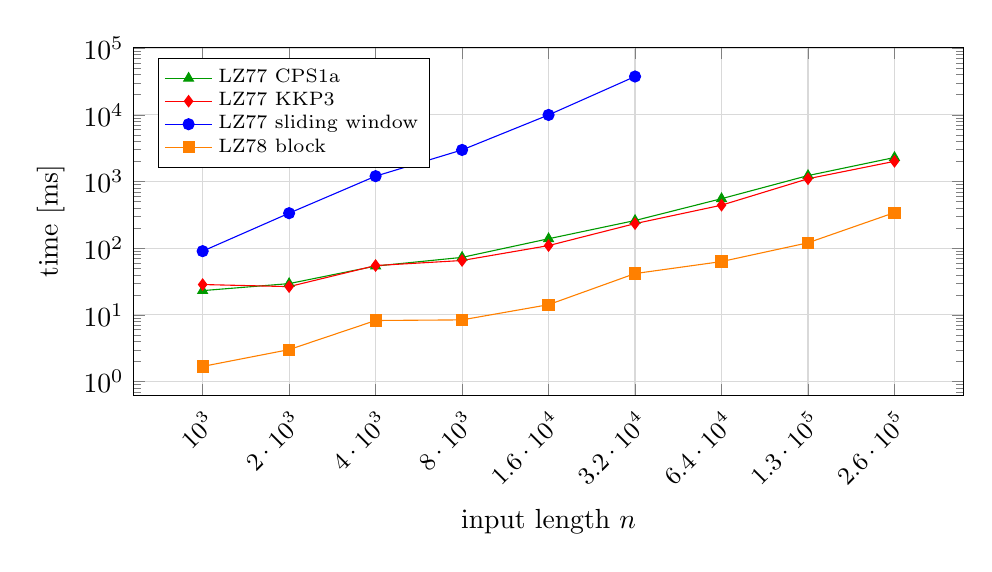
\begin{tikzpicture}
\begin{axis}[
  width = \linewidth, height = 6cm,
  xlabel = {input length $n$}, ylabel = {time [ms]},
  xmode = log, ymode = log,
  legend pos = north west, legend cell align = left,
  legend style = {font = \scriptsize, row sep = -2pt, inner sep = 2pt},
  xmajorgrids = true, ymajorgrids = true,
  xminorgrids = false, yminorgrids = false,
  minor tick num = 0,
  grid style = {draw = gray!30},
  xtick = {1000, 2000, 4000, 8000, 16000, 32000, 64000, 128000, 256000},
  xticklabels = {$10^{3}$, $2 \cdot 10^{3}$, $4 \cdot 10^{3}$, $8 \cdot 10^{3}$, $1.6 \cdot 10^{4}$, $3.2 \cdot 10^{4}$, $6.4 \cdot 10^{4}$, $1.3 \cdot 10^{5}$, $2.6 \cdot 10^{5}$},
  x tick label style = {rotate = 45, anchor = north east, font = \small},
]
\addplot[color = green!60!black, mark = triangle*] coordinates {(1000, 23.15) (2000, 29.49) (4000, 54.04) (8000, 72.95) (16000, 138.71) (32000, 260.41) (64000, 553.19) (128000, 1228.74) (256000, 2293.59)};
\addlegendentry{LZ77 CPS1a}
\addplot[color = red, mark = diamond*] coordinates {(1000, 28.57) (2000, 26.58) (4000, 54.98) (8000, 65.49) (16000, 109.56) (32000, 233.9) (64000, 442.13) (128000, 1101.65) (256000, 2008.58)};
\addlegendentry{LZ77 KKP3}
\addplot[color = blue, mark = *] coordinates {(1000, 90.41) (2000, 335.41) (4000, 1204.21) (8000, 2978.29) (16000, 9966.61) (32000, 37584.71)};
\addlegendentry{LZ77 sliding window}
\addplot[color = orange, mark = square*] coordinates {(1000, 1.69) (2000, 3.02) (4000, 8.25) (8000, 8.43) (16000, 14.25) (32000, 41.72) (64000, 63.12) (128000, 120.72) (256000, 342.32)};
\addlegendentry{LZ78 block}
\end{axis}
\end{tikzpicture}
\captionof{figure}{random binary, encoding time.}
\label{fig:random-binary-encoding}
\end{center}

\begin{center}
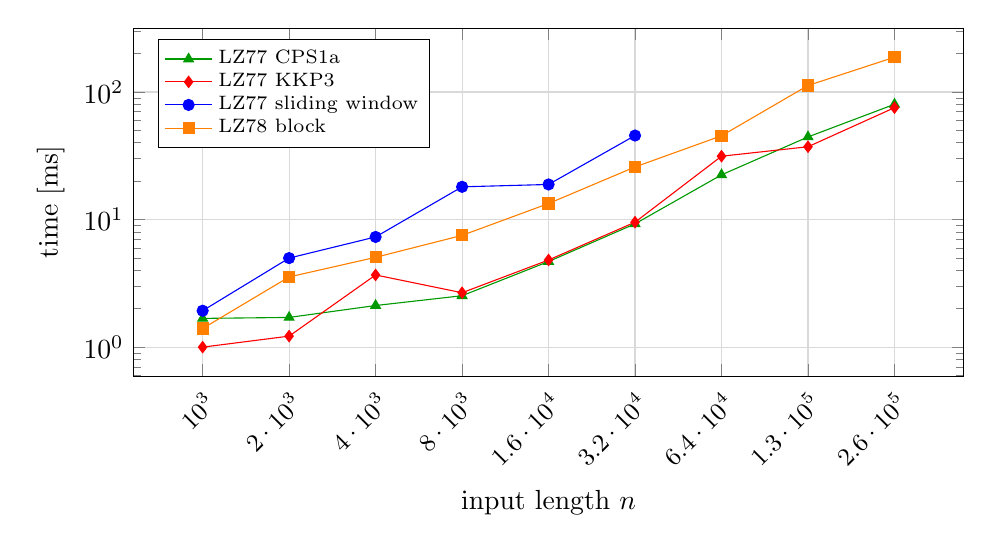
\begin{tikzpicture}
\begin{axis}[
  width = \linewidth, height = 6cm,
  xlabel = {input length $n$}, ylabel = {time [ms]},
  xmode = log, ymode = log,
  legend pos = north west, legend cell align = left,
  legend style = {font = \scriptsize, row sep = -2pt, inner sep = 2pt},
  xmajorgrids = true, ymajorgrids = true,
  xminorgrids = false, yminorgrids = false,
  minor tick num = 0,
  grid style = {draw = gray!30},
  xtick = {1000, 2000, 4000, 8000, 16000, 32000, 64000, 128000, 256000},
  xticklabels = {$10^{3}$, $2 \cdot 10^{3}$, $4 \cdot 10^{3}$, $8 \cdot 10^{3}$, $1.6 \cdot 10^{4}$, $3.2 \cdot 10^{4}$, $6.4 \cdot 10^{4}$, $1.3 \cdot 10^{5}$, $2.6 \cdot 10^{5}$},
  x tick label style = {rotate = 45, anchor = north east, font = \small},
]
\addplot[color = green!60!black, mark = triangle*] coordinates {(1000, 1.68) (2000, 1.71) (4000, 2.12) (8000, 2.53) (16000, 4.69) (32000, 9.26) (64000, 22.42) (128000, 44.45) (256000, 80.11)};
\addlegendentry{LZ77 CPS1a}
\addplot[color = red, mark = diamond*] coordinates {(1000, 1.0) (2000, 1.22) (4000, 3.68) (8000, 2.67) (16000, 4.82) (32000, 9.54) (64000, 31.38) (128000, 37.24) (256000, 75.35)};
\addlegendentry{LZ77 KKP3}
\addplot[color = blue, mark = *] coordinates {(1000, 1.93) (2000, 4.99) (4000, 7.31) (8000, 18.06) (16000, 18.85) (32000, 45.58)};
\addlegendentry{LZ77 sliding window}
\addplot[color = orange, mark = square*] coordinates {(1000, 1.4) (2000, 3.55) (4000, 5.06) (8000, 7.52) (16000, 13.36) (32000, 25.85) (64000, 45.36) (128000, 112.46) (256000, 187.37)};
\addlegendentry{LZ78 block}
\end{axis}
\end{tikzpicture}
\captionof{figure}{random binary, decoding time.}
\label{fig:random-binary-decoding}
\end{center}

\begin{center}
\begin{tabular}{lrrrrrr}
\hline
algorithm & $n$ & $\alpha$ & $z$ & $\rho$ & encode [ms] & decode [ms] \\
\hline
LZ77 sliding window & 32000 & 2 & 2175 & 2.107 & 37815.84 & 34.95 \\
LZ78 block & 32000 & 2 & 3218 & 1.1793 & 26.11 & 22.39 \\
LZ77 CPS1a & 32000 & 2 & 2175 & 1.4273 & 255.39 & 9.09 \\
LZ77 KKP3 & 32000 & 2 & 2175 & 1.4273 & 220.57 & 10.32 \\
\hline
\end{tabular}
\captionof{table}{random binary: uniform over two letters.}
\label{tab:random-binary}
\end{center}